%!TEX root = ../thesis.tex
%*******************************************************************************
%****************************** Second Chapter *********************************
%*******************************************************************************

\chapter{Background}

\ifpdf
    \graphicspath{{Chapter2/Figs/Raster/}{Chapter2/Figs/PDF/}{Chapter2/Figs/}}
\else
    \graphicspath{{Chapter2/Figs/Vector/}{Chapter2/Figs/}}
\fi


\section{Concrete}
\subsection{Rheology}

Rheology is defined as study of the flow of a material under an applied shear stress. Developing an understanding of the rheological properties is therefore paramount when attempting to model a process requiring a flowable medium. A method for obtaining this understanding is presented herein.\\
\newline
\noindent
\citet{Sperwall} like many other British and European standards refer to concrete in terms of 'workability' and 'consistence'; qualitative terms used to empirically describe the rheological properties of concrete. It is, however, accepted that although these terms are long-standing \citep{Tattersall83}, they may not be the most appropriate due to their subjectiveness. \citet{Tattersall90} presented the possibility of using a more quantitative approach to analysing concrete, namely the Bingham model, {\bfseries eq. \ref{eq:bingham}}.
\begin{equation}
\tau = \mu\dot{\gamma}+\tau_0
\label{eq:bingham}
\end{equation}

\noindent
$\tau$ represents the shear stress $[Pa]$, $\mu$ represents plastic viscosity [Pa] and $\dot{\gamma}$ represents the shear rate $[s^-1]$. It is known that fresh tremie concrete at rest requires a force in order to initiate flow. This required shear stress to initiate flow can be termed yield stress, $\tau_0$. The relationship of each is demonstrated in {\bfseries figure \ref{fig:bingham}}
\begin{figure}[H]
\centering
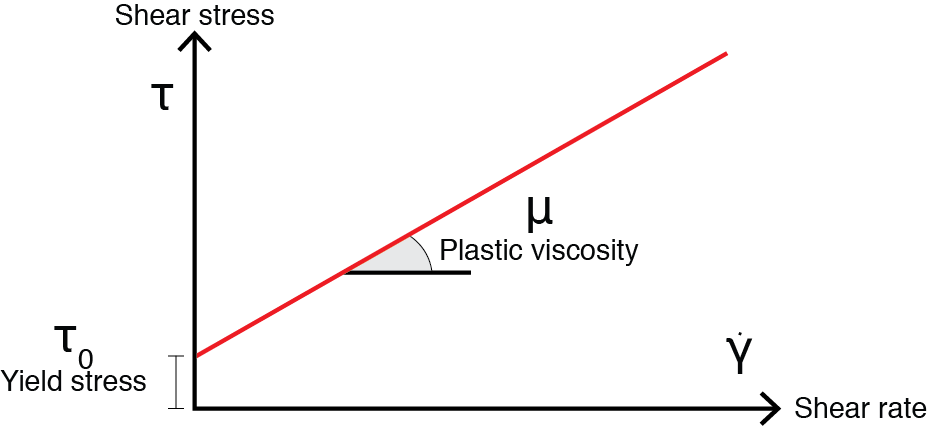
\includegraphics[width=0.8\textwidth]{bingham.png}
\caption{\label{fig:bingham} Relationship of Bingham parameters.}
\end{figure}

%************************************ TESTING*********************************************
\subsection{Measurement Techniques for Fresh Concrete}
Tests determining properties of concrete are used substantially on-site with much credit given to the results; potentially leading to concrete batches being prevented from use. Tests are designed to assess two key aspects of a concrete; Consistence and Stability. Consistence refers to the flowability of a concrete and stabilty refers to the ability of a concrete to resist segregation \citep{Sperwall}.There are numerate accepted concrete tests, the aim of each being to target a  property and assess its impact.\\
\newline
\noindent
Focusing on the rheological parameters often poses difficulties for tests traditionally designed to provide empirical data. One of such tests is the popular L-box test (\citeauthor{BS1235010}) {\bfseries figure \ref{fig:lbox}}. Originally developed to asses super workable concrete \citep{lboxaus} the test is designed such that it assess key aspects of what is presumed to be a suitable concrete; passing ability, free surface flow, and dynamic segregation \citep{NGUYEN06}.\\
\newline
\noindent
Concrete is placed in the vertical portion of the apparatus and filled, whilst a gate maintains a division between the vertical and horizontal segments. Once opened, the gate allows concrete to flow freely into the horizontal segment, first passing through rebars with a width determined by the largest aggregate. The result of this test is therefore governed by both rheology and the concretes ability to maintain heterogeneity \citep{karsten}.\\
\begin{figure}[H]
\centering
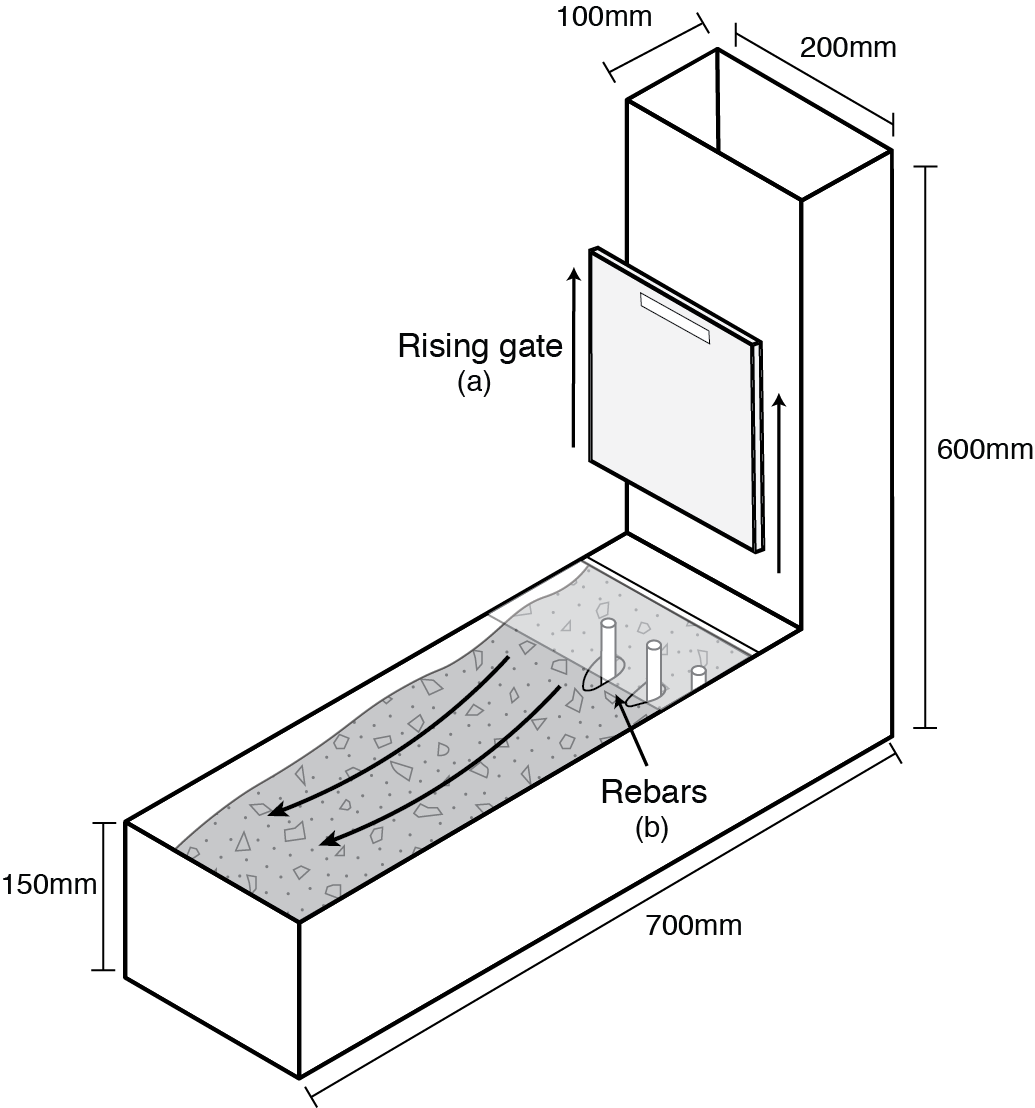
\includegraphics[width=0.7\textwidth]{lbox.png}
\caption{\label{fig:lbox} L-box test apparatus. a) Rising gate to initiate concrete flow) b) Rebars to test dynamic segregation and passing ability}
\end{figure}
\noindent
Segregation within concrete is defined by the measured concretes ability to maintain uniformity against forces applied during emplacement (dynamic segregation) and when the concrete is at rest (static segregation) \citep{turgut12}, {\bfseries figure \ref{fig:hvsi}}. \citet{mouret08} stresses the importance of developing a test with the ability to determine the segregation propensity of a concrete. The passing of concrete through the bars offers an important dynamic segregation indicator, but the indications of yield stress and plastic viscosity are inconclusive, \citet{karsten}.\\
\newline
\noindent
For concrete placement by tremie in submerged condition under support fluid, \citet{Sperwall} recommends the use of the 'slump-flow' test in accordance with \citeauthor{BS123508} as one way to measure of the consistence of a concrete, ensuring it is workable enough for the tremie process. {\bfseries figure \ref{fig:lbox}a} demonstrates how a slump test is designed. Widely attributed to have originated from Abrams \citep{graf33}, the test has maintained its position as one of the most important throughout the industry \citep{bartos02} in part due it its repeatability and practicality, \citeauthor{BS123508}. In slump testing, a flat-topped cone mould is filled with concrete to be tested and allowed to rest. The mould is then raised with constant velocity. The slump is defined as the difference between the height of the mould and the height of the slumped material after flow stops. An alternative, but more common measurement for tremie concrete is a measure of the final spread diameter of the material, the slump-spread, {\bfseries figure \ref{fig:slumptest}a} \citep{GAO15}.\\
\begin{figure}[H]
\centering
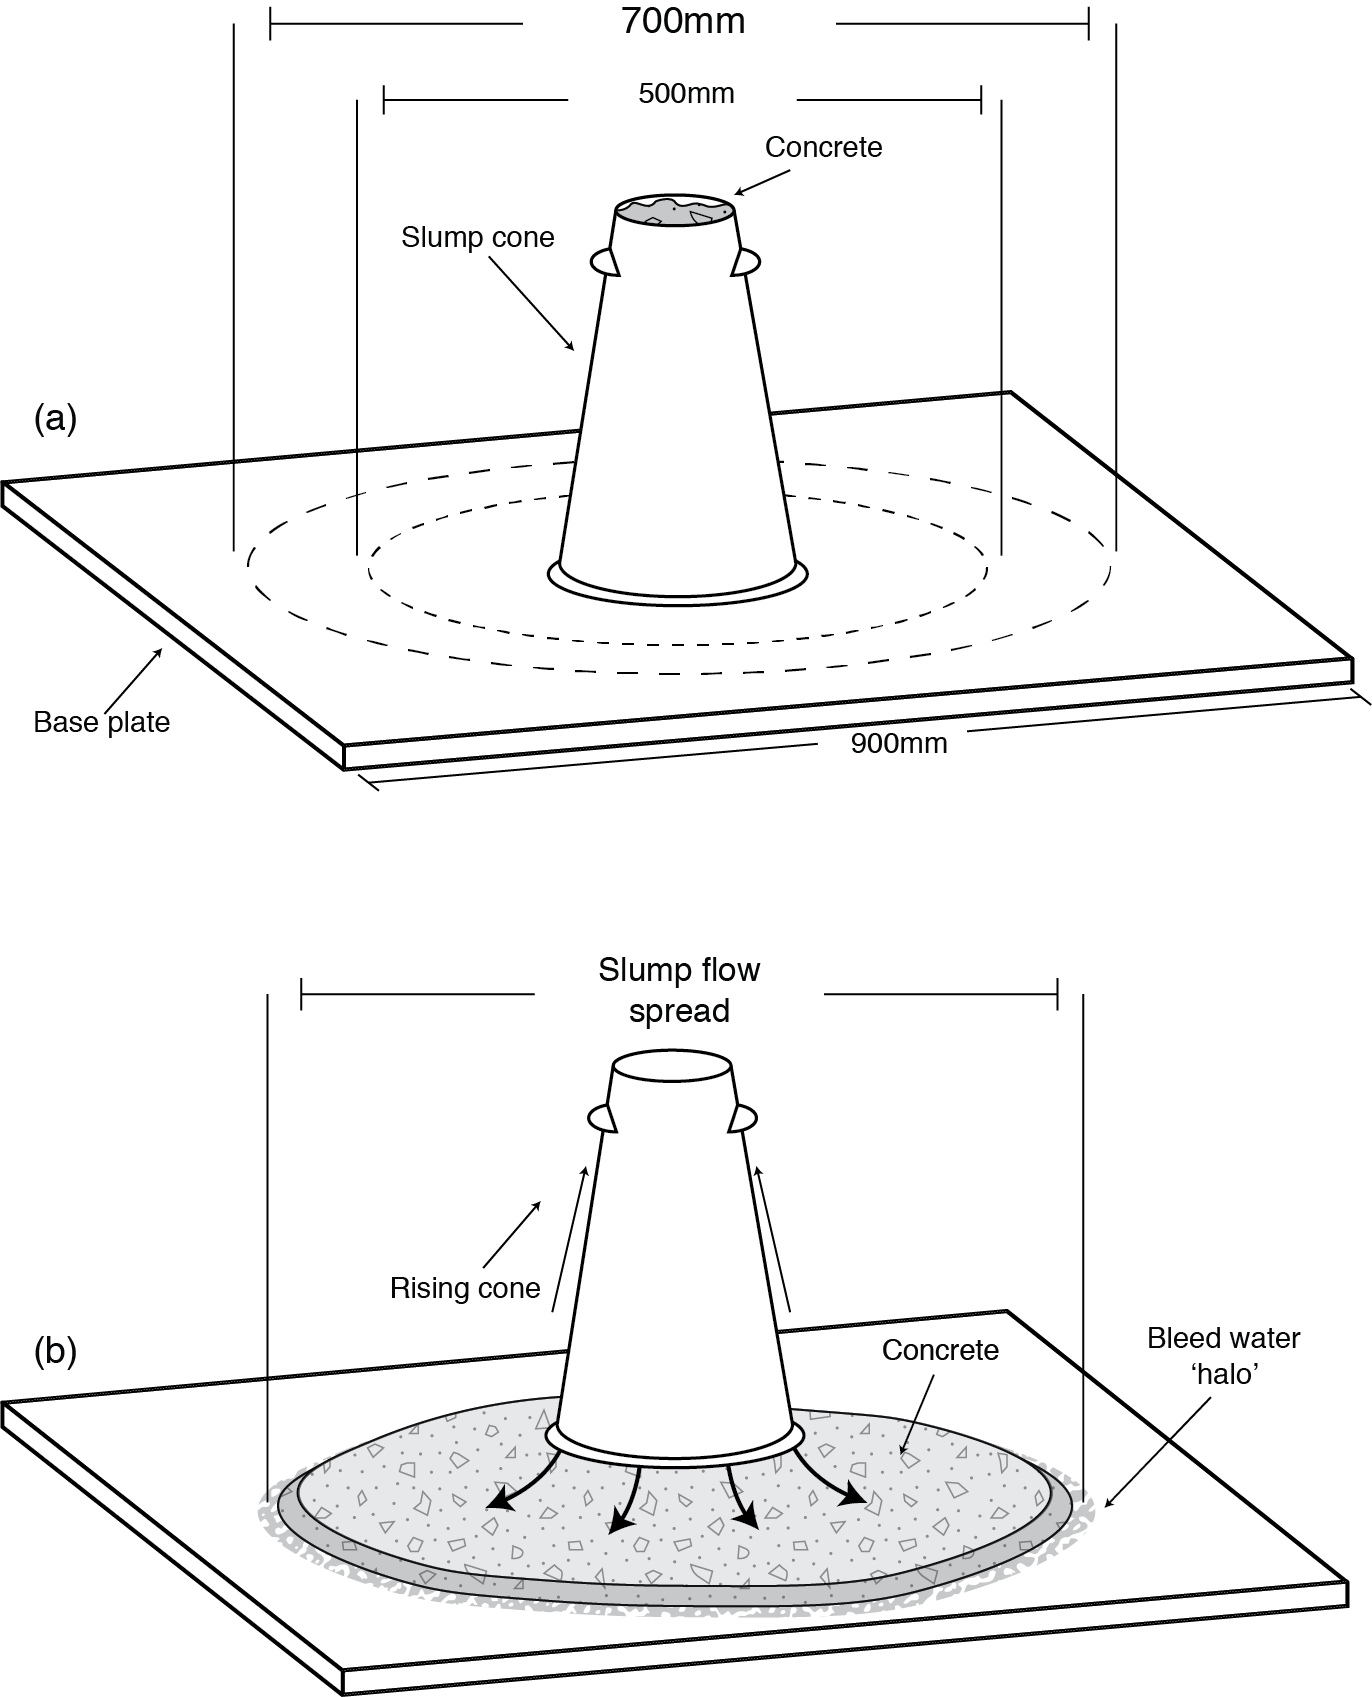
\includegraphics[width=0.85\textwidth]{slumptest.png}
\caption{\label{fig:slumptest} a) Slump-flow test apparatus in accordance with BS EN 12350-8. b) Visualisation of slump spread and segregation halo.}
\end{figure}
\noindent
Owing to the central role of segregation in concrete performance, one popular method used in conjunction with a slump flow test is based on the visual stability index (VSI) of the slump flow \citep{VSI}. By identifying the presence of a mortar halo around the slump-spread and rating its extensiveness visually from 0 to 3, an assessment of the stability can be quantified \citep{pci03}. A 0 rating represents no segregation and a rating of 3 represents severe segregation.\\
\newline
\noindent
However, visual evaluation of bleeding and aggregate segregation according to the VSI test may be misleading, as only dynamic stability evaluations can be made. Dynamic segregation occurs in both horizontal and vertical directions. Vertical segregation results in less aggregate within top layers of the flowing concrete and horizontal results in loss of aggregate at the flow front \citep{HOSSEI17}. \citet{TREGGER12} demonstrated the slump-flow test to be only capable of indicating horizontal dynamic segregation resistances. Mixtures that segregate during slump flow would likely segregate after placement, but the lack of segregation during a slump flow test does not necessarily imply that the mixture is resistant to static segregation \citep{bonen05}.
\\
\\
\begin{figure}[H]
\centering
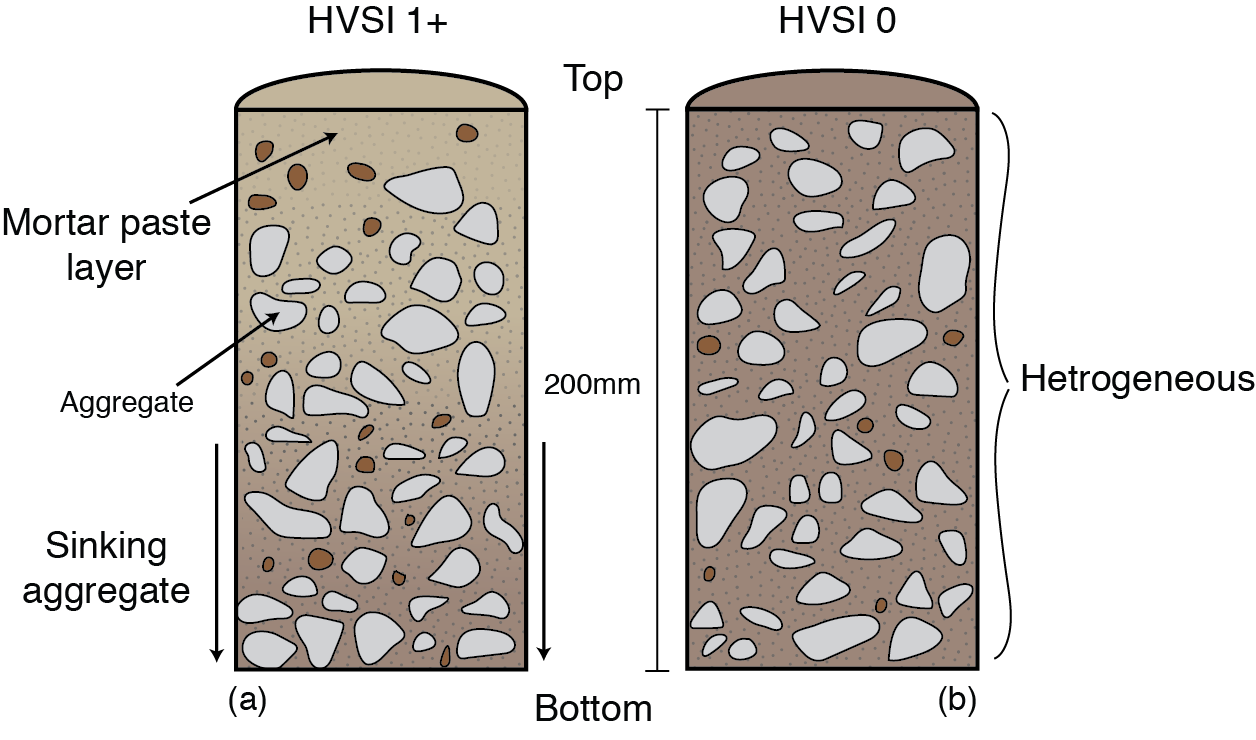
\includegraphics[width=0.9\textwidth]{hvsi.png}
\caption{\label{fig:hvsi} Demonstration of static segregation within a Hardened Visual Stability Index test. a) Segregation occurring, b) no segregation.}
\end{figure}
\noindent
One method for obtaining an indication of static segregation is the Static Segregation Test in accordance with \citeauthor{HVSI}. The test involves a cylindrical sample of the test concrete allowed to cure over time. It is then sawn in half and an assessment of the level of segregation rated form 0-3, similar to a VSI scale; referred to as the Hardened Visual Stability Index HVSI) {\bfseries figure \ref{fig:hvsi}}. Although this test does not provide instant feedback prior to a mix being used on-site, for laboratory mix designing, it highlights the susceptibility of a mix to undergo static segregation. Segregation of any kind can cause the reduction of strength properties of concrete.\\
\newline
\noindent
In association with segregation, bleed is often discussed. Where segregation refers to the loss of heterogeneity of a concrete, bleed refers to the loss of water or paste of a concrete. The most common bleed test is in accordance with \citeauthor{ASTMbleed} where a sample of concrete is allowed to rest and surface water content measured, to assess the level of water-loss or 'bleed' of the concrete. Bleed is often referred to as analogous to segregation, in that they both represent a separation of the concrete into constitutive elements; causing detriment to concrete strength properties.\\
\newline
\noindent
A recent attempt to predict the water retention ability of concrete was raised in \citet{CIA} in the form of the BAUER Filtration test. Although not currently under a design code standard, the test is becoming more common throughout the industry \cite{Sperwall}. The test simulates concrete under hydrostatic pressure and determines the loss of water using a filter. Measured water loss in the form of filtrate determines if concrete at the base of a pile undergoing hydrostatic pressure increases from an increasing weight above will bleed, and likely segregate.\\
\newline
\noindent
\citet{wallevik06} criticises the use of using single value workability tests on the grounds that two concretes of different rheological parameters may produce the same result. An alternative approach is offered in the literature to draw physical quantities from these simple tests. \citet{roussel50} and \citet{wallevik06} attempt to correlate final slump measurements with the initial yield stress, using experimental results to derive equations; producing reliable results. Both papers however, neglect the impact of plastic viscosity on the final slump diameter. \citet{sofcf} state that at low shear stresses where the stopping and starting is of interest, such as a slump flow test, yield stress is the main contributing factor.\\
\begin{figure}[H]
\centering
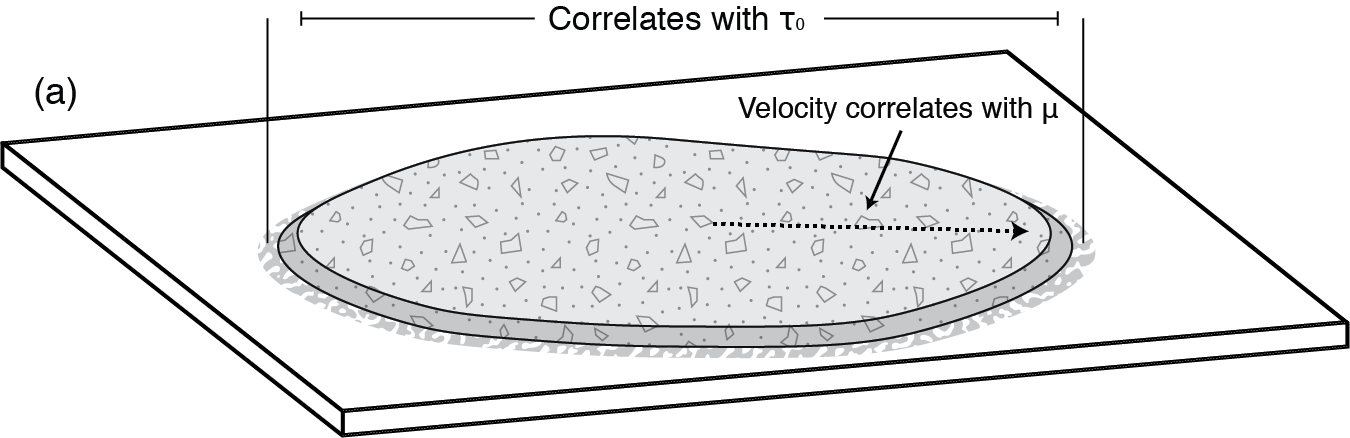
\includegraphics[width=0.9\textwidth]{tau.png}
\caption{\label{fig:tau} a) Correlation of slump spread to Bingham parameters.}
\end{figure}
\noindent
\citet{wallevik06} concluded that no correlation between final slump and plastic viscosity could be confidently made. Conversely, \citet{TUM,BOUVET10} both observed the velocity at which the slump proceeds has a clear correlation with plastic viscosity {\bfseries figure \ref{fig:tau}}.\\
\newline
\noindent
By using experimentally derived parameters ($\mu$ \& $\tau_0$) as inputs for a Bingham constitutive model, the resultant slump diameter and plastic viscosity can be cross referenced with expected values as a potential means to validate a model.\\
\newline
One caveat to using a simple Bingham model is the neglection of the observed thixotropic effect of fresh tremie concrete. A thixotropic concrete has a reversible stiffening effect active when at rest \citep{EFFC}. As time increases, so does $\tau_0$. \citet{roussel06} offered a potential mathematical solution, a flocculation state $\lambda$ is incorporated into the existing Bingham model, {\bfseries eq. \ref{eq:thix}}. Such that $A_{thix}$ is the re-structuration rate at rest ($0.1-2 Pa$) and $\alpha$ is the destruction parameter (typical values of the order $0.01$) {\bfseries eq. \ref{eq:thixdt}}, \citet{roussel07}.
\begin{equation}
\tau = \mu\dot{\gamma}+(1+\lambda)\tau_0
\label{eq:thix}
\end{equation}

\begin{equation}
\therefore
\frac{\partial \lambda}{\partial t}=\frac{A_{thix}}{\tau_0}-\alpha\lambda\dot{\gamma}
\label{eq:thixdt}
\end{equation}
\\
\citet{roussel07} observed that for time-scales relating to concrete measurement techniques, thixotropic effects are marginal. However when considering a pile-scale problem, thixotropic increases in yield stress become increasingly important.\\
\newline
\begin{figure}[H]
\centering
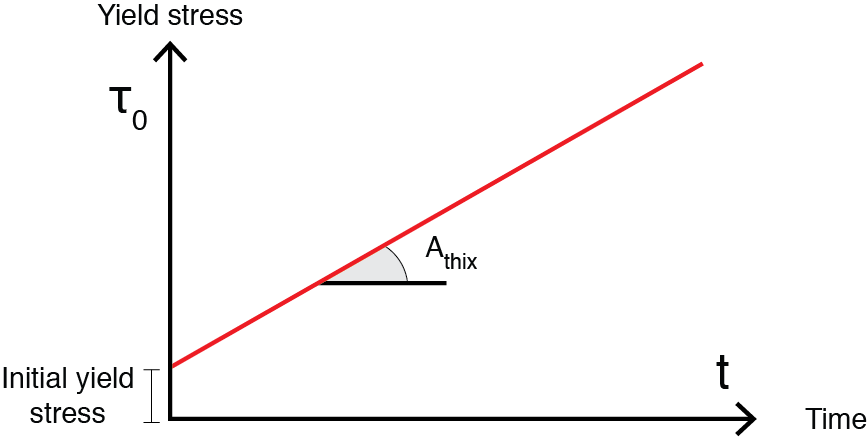
\includegraphics[width=0.8\textwidth]{thix.png}
\caption{\label{fig:thix} Relationship of Thixotropy parameters.}
\end{figure}
\noindent
In summary, \citet{Sperwall} offer a range of concrete testing methods, designed to attribute a quantitative measurements to traditionally empirical tests. These range from tests designed to assess the 'passing ability' of concrete \citeauthor{BS1235010}, to those designed to measure segregation of concrete into its constituent materials \citeauthor{ASTMbleed}. Whilst these tests do not offer the level of information provided by the slump flow, they must not be neglected as there is still much to be gained by analysing how known test results compare with a simulated version.
%********************************** AOI  ****************************
\section{Areas of Investigation}
A review of current guidelines on the tremie process is presented here, with reference made to how each guideline has an impact on the process. Reference is also made to how each issue raised may have an impact on the final functionality of the foundation.

\subsection{Initiation of Concrete Flow}
Areas of investigation related to the initiation of concrete flow are centred around the physical apparatus used in the process and the conditions of the shaft prior to beginning concreting as seen in {\bfseries figure \ref{fig:flow_init}}.\\

\noindent
The importance of base cleaning, demonstrated in {\bfseries figure \ref{fig:flow_init}a}, is reiterated throughout \citeauthor{BS1536}, \citetex{EFFC}, and \citetex{Sperwall}. The need for pile baring capacity to be accurately calculated by relying on the assumption of a smooth base being a primary concern. However, although a smooth base is critical for some pile design purposes it is note for all. \citetex{EFFC} hypothesise that debris from the base can be stirred up and included in the pile if the base is left unclean. Developing a simulation to assess the degree of inclusions caused by an unclean base could provide advice on whether base cleaning is needed in conditions where end baring capacity is not a critical factor of the pile design.\\

\noindent
{\bfseries
Figure \ref{fig:flow_init}b} and {\bfseries figure \ref{fig:flow_init}c}  demonstrate the initial charging and raising of the tremie to initiate concrete flow. \citetex{Sperwall} recommend raising the pipe to $200mm$ prior to initiation of flow to allow for the prevention of blockages from the initial pour. Both \citetex{Sperwall} and \citetex{EFFC} also recommend the use of a plug to allow the tremie to be filled with concrete prior to initiation. This also allows for the prevention of contamination with support fluid during filling of the pipe. However, little evidence is provided to determine the effectiveness of using such a method. This study aims to simulate varying plugging methods and make a recommendation on the effectiveness of each.\\

\noindent
Finally, {\bfseries figure \ref{fig:flow_init}d}  demonstrates the first 'cut' of the tremie pipe. During concreting, the tremie pipe is periodically raised and a segment unscrewed. This maintains a required embedment of around $3m-8m$ (\citeauthor{BS1536}) throughout the pouring process. In contrast, \citetex{EFFC} recommend for the first cut, an embedment of $5m$ is maintained. Analysing the behaviour of concrete with these contrasting embedment depths can help alleviate some of the contrasting opinions currently surrounding the depth of embedment. Additionally, \citetex{EFFC} and \citetex{Sperwall} also make reference to maintaining a charged pipe such that the hydrostatic pressure inside the pipe is greater than that outside, preventing inflow of the support fluid. Observations of pressure changes within the tremie pipe will be made during the simulation to assess the likelihood of infiltration of support fluid into the tremie pipe.

\begin{figure}[H]
\centering
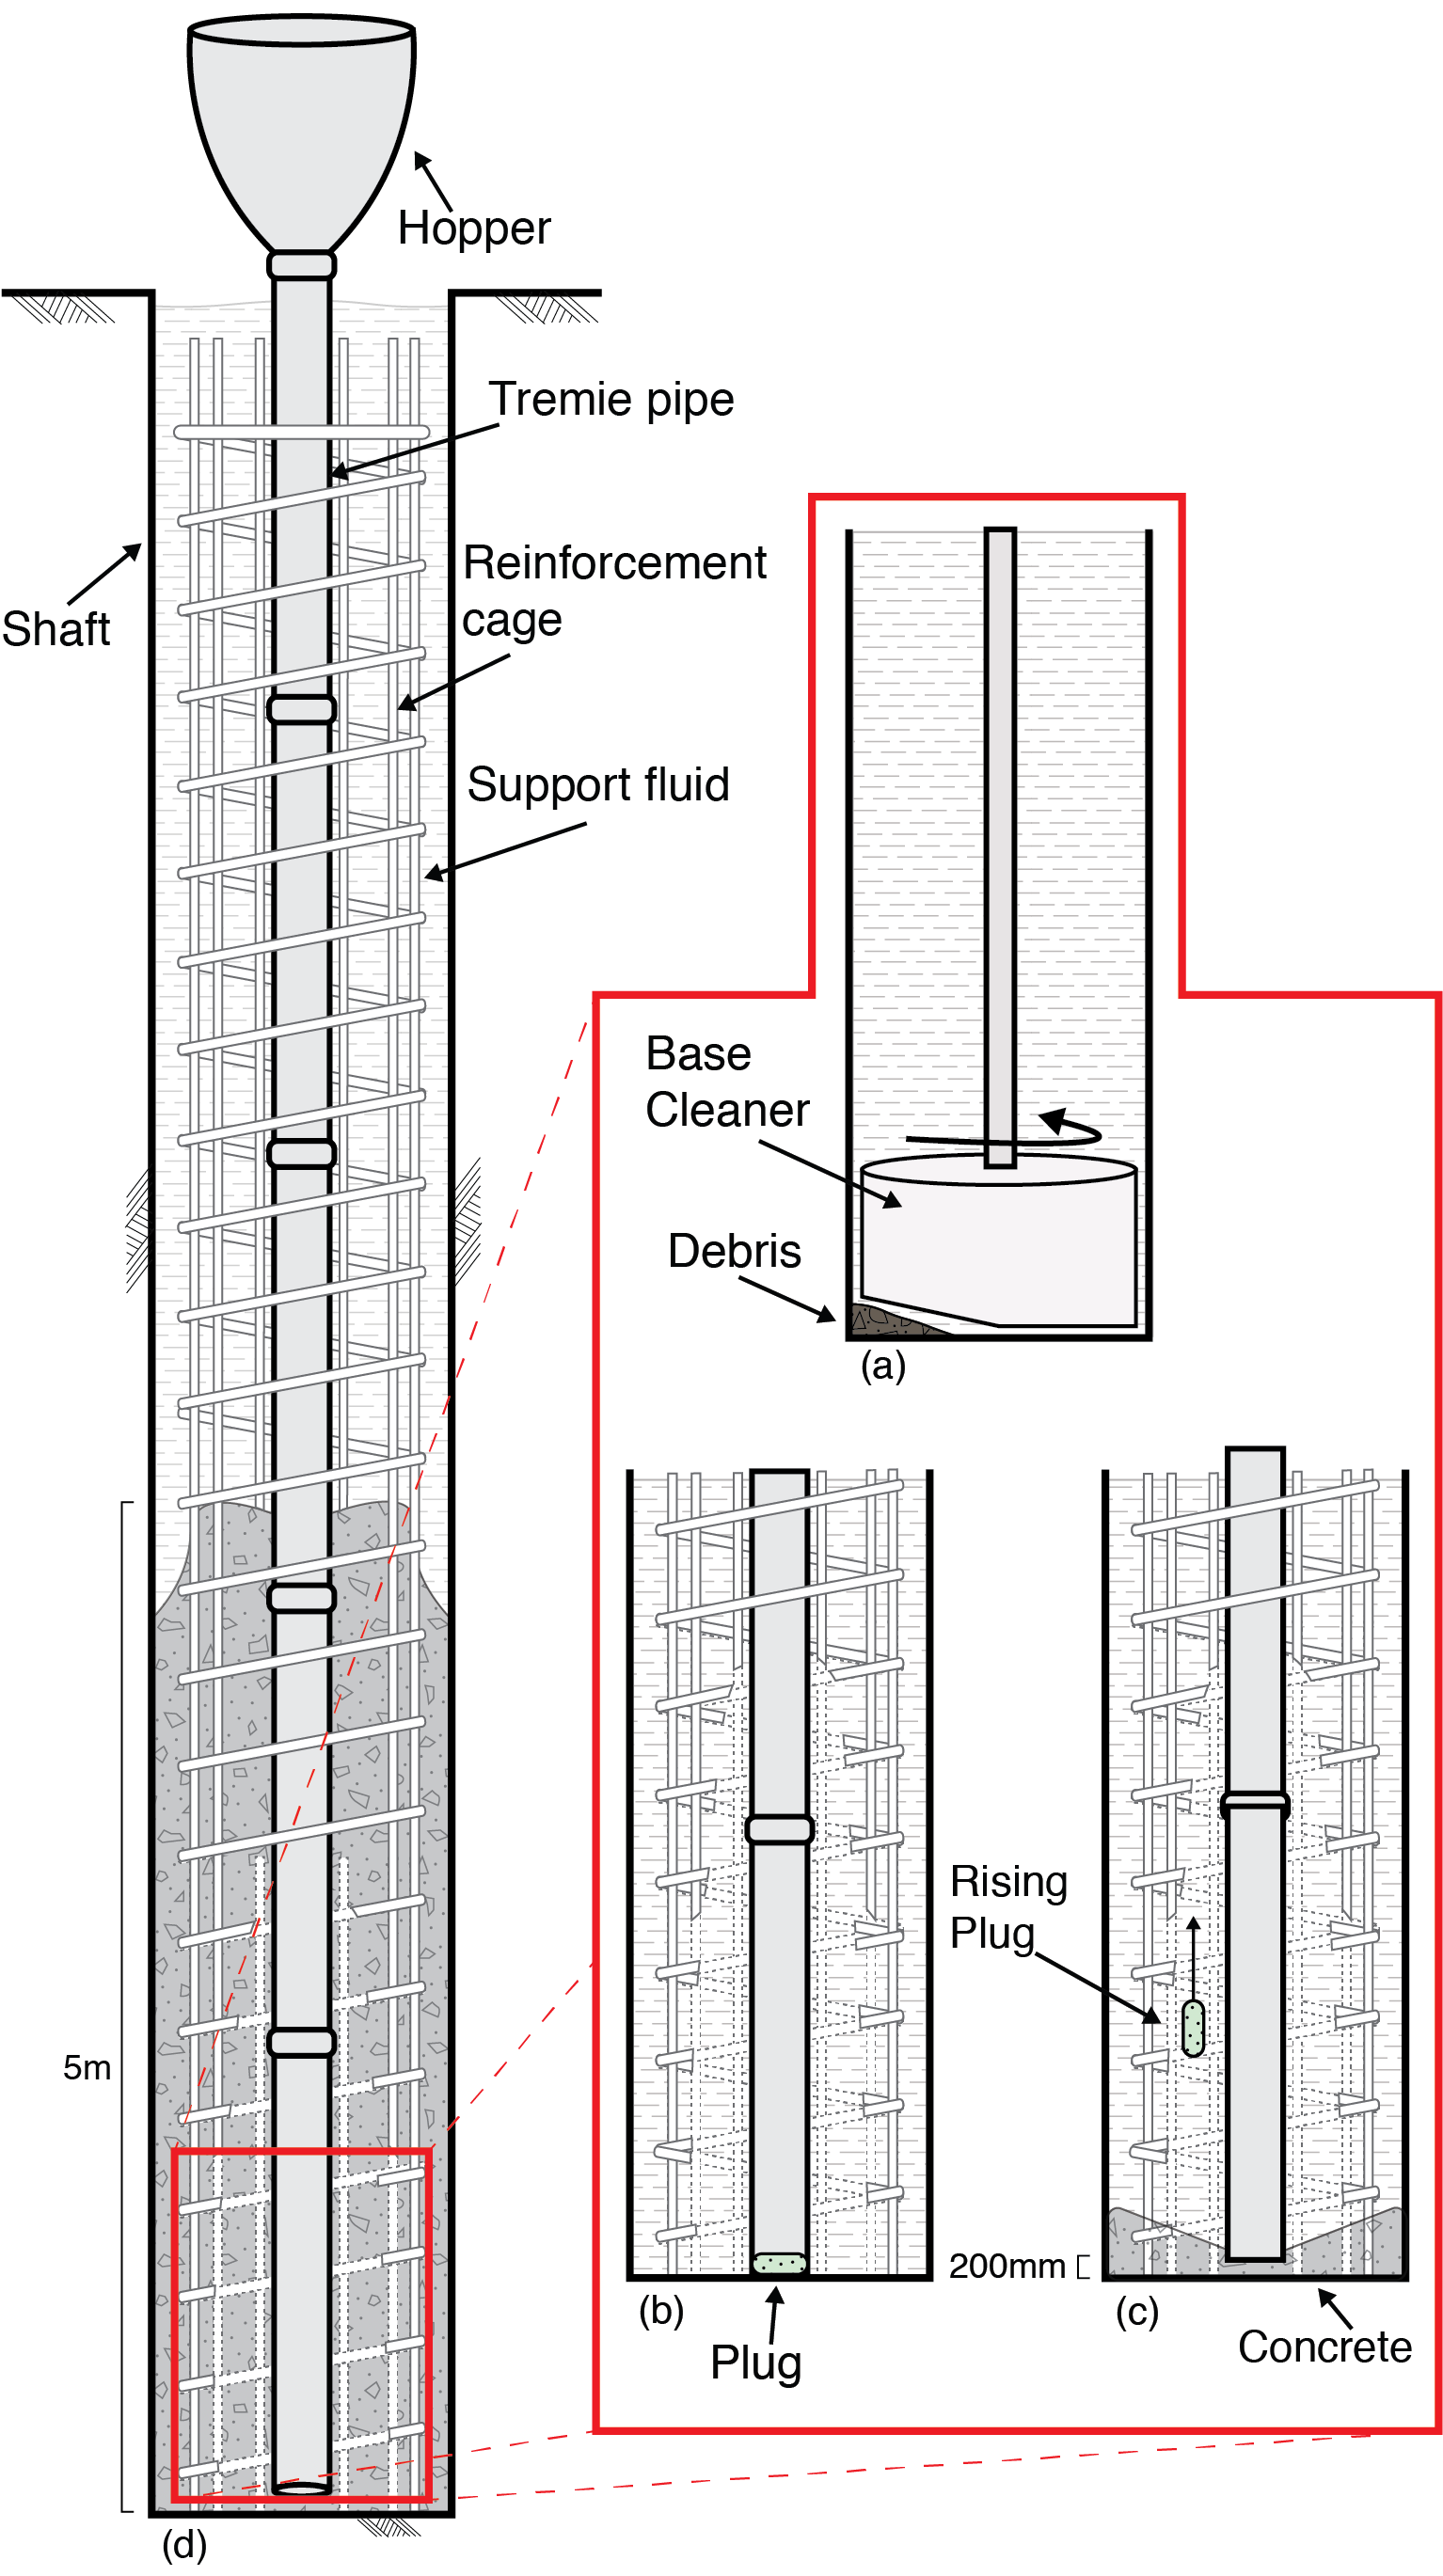
\includegraphics[width=0.8\textwidth]{initial_flow_issues.png}
\caption{\label{fig:flow_init} a) Schematic of base cleaner tool used to create a smooth base in shaft. b)\& c) Schematic showing use of plug or 'pig' to prevent concrete within pipe from free-falling into support fluid. d) Schematic showing required embedment before tremie can be raised.}
\end{figure}

%********************************** During Flow  ****************************
\subsection{During Concrete Flow}

During initiation of flow problems are likely to arise as a result of improper concreting techniques, the same cannot be said for issues that arise during concrete flow; for these issues are more closely related to the material properties of the concrete.\\

\noindent
\citetex{Sperwall} and \citetex{EFFC} emphasise that concrete should flow freely from the tremie pipe without the need for surging (lowering and raising the pipe to facilitate flow). Although flowing freely is a requirement, little is understood about the manner in which the concrete flows. \citetex{EFFC} describes the the various theorised methods of the flowing of concrete out of the tremie pipe and into the surrounding shaft as varying 'flow patterns'. There are two main theorised flow patterns, 'plug flow' and 'volcano flow' as demonstrated in {\bfseries figure XX}. Each flow pattern has an impact on the required open-life of the concrete; plug flow requiring the lengthier open-life. Achieving a longer open life requires the potential introduction of superplasticizers and retarders, both of which come at an increased cost and often a lack of understanding. Therefore, determining the dominant flow pattern through simulations could help provide advice on concrete open-life.\\

\noindent
A congested reinforcement cage can give rise to poor coverage of concrete, in contrast there are cases where a seemingly uncongested cage has induced a defect termed 'matressing'. This occurs as a result of concrete poorly flowing around the rebars of a reinforcement cage, as demonstrated in {\bfseries figure \ref{fig:matress}a \& b}. \citet{EFFC} infer the implications of such imperfections could cause pathways bleed water, reductions in bearing capacity, and durability concerns. Developing a series of simulations to predict the likelihood of matressing occurring will generate useful insights into both how reinforcement cages are designed and how important the material properties of the concrete are in reducing matressing.It is also suggested that a reduction in hydrostatic pressure towards the top of the pile may exacerbate this problem, which will be investigated.\\

\noindent
\citeauthor{BS1536} recommends the use of a support fluid such as bentonite for preventing collapse of the shaft during drilling and casting of foundations. Although a fundamental part of the casting in situ process, it is not without complications, {\bfseries figure \ref{fig:matress}c}. It is observed during casting that atop the rising concrete with the pile will be an interface layer; a mixture of support fluid and concrete. This low strength material could possibly be enveloped by concrete to form an inclusion, particularly in the cover zone. Investigating how this material flows through a pile may shed light on what is currently a poorly understood by-product of using bentonite support fluid. 


\begin{figure}[H]
\centering
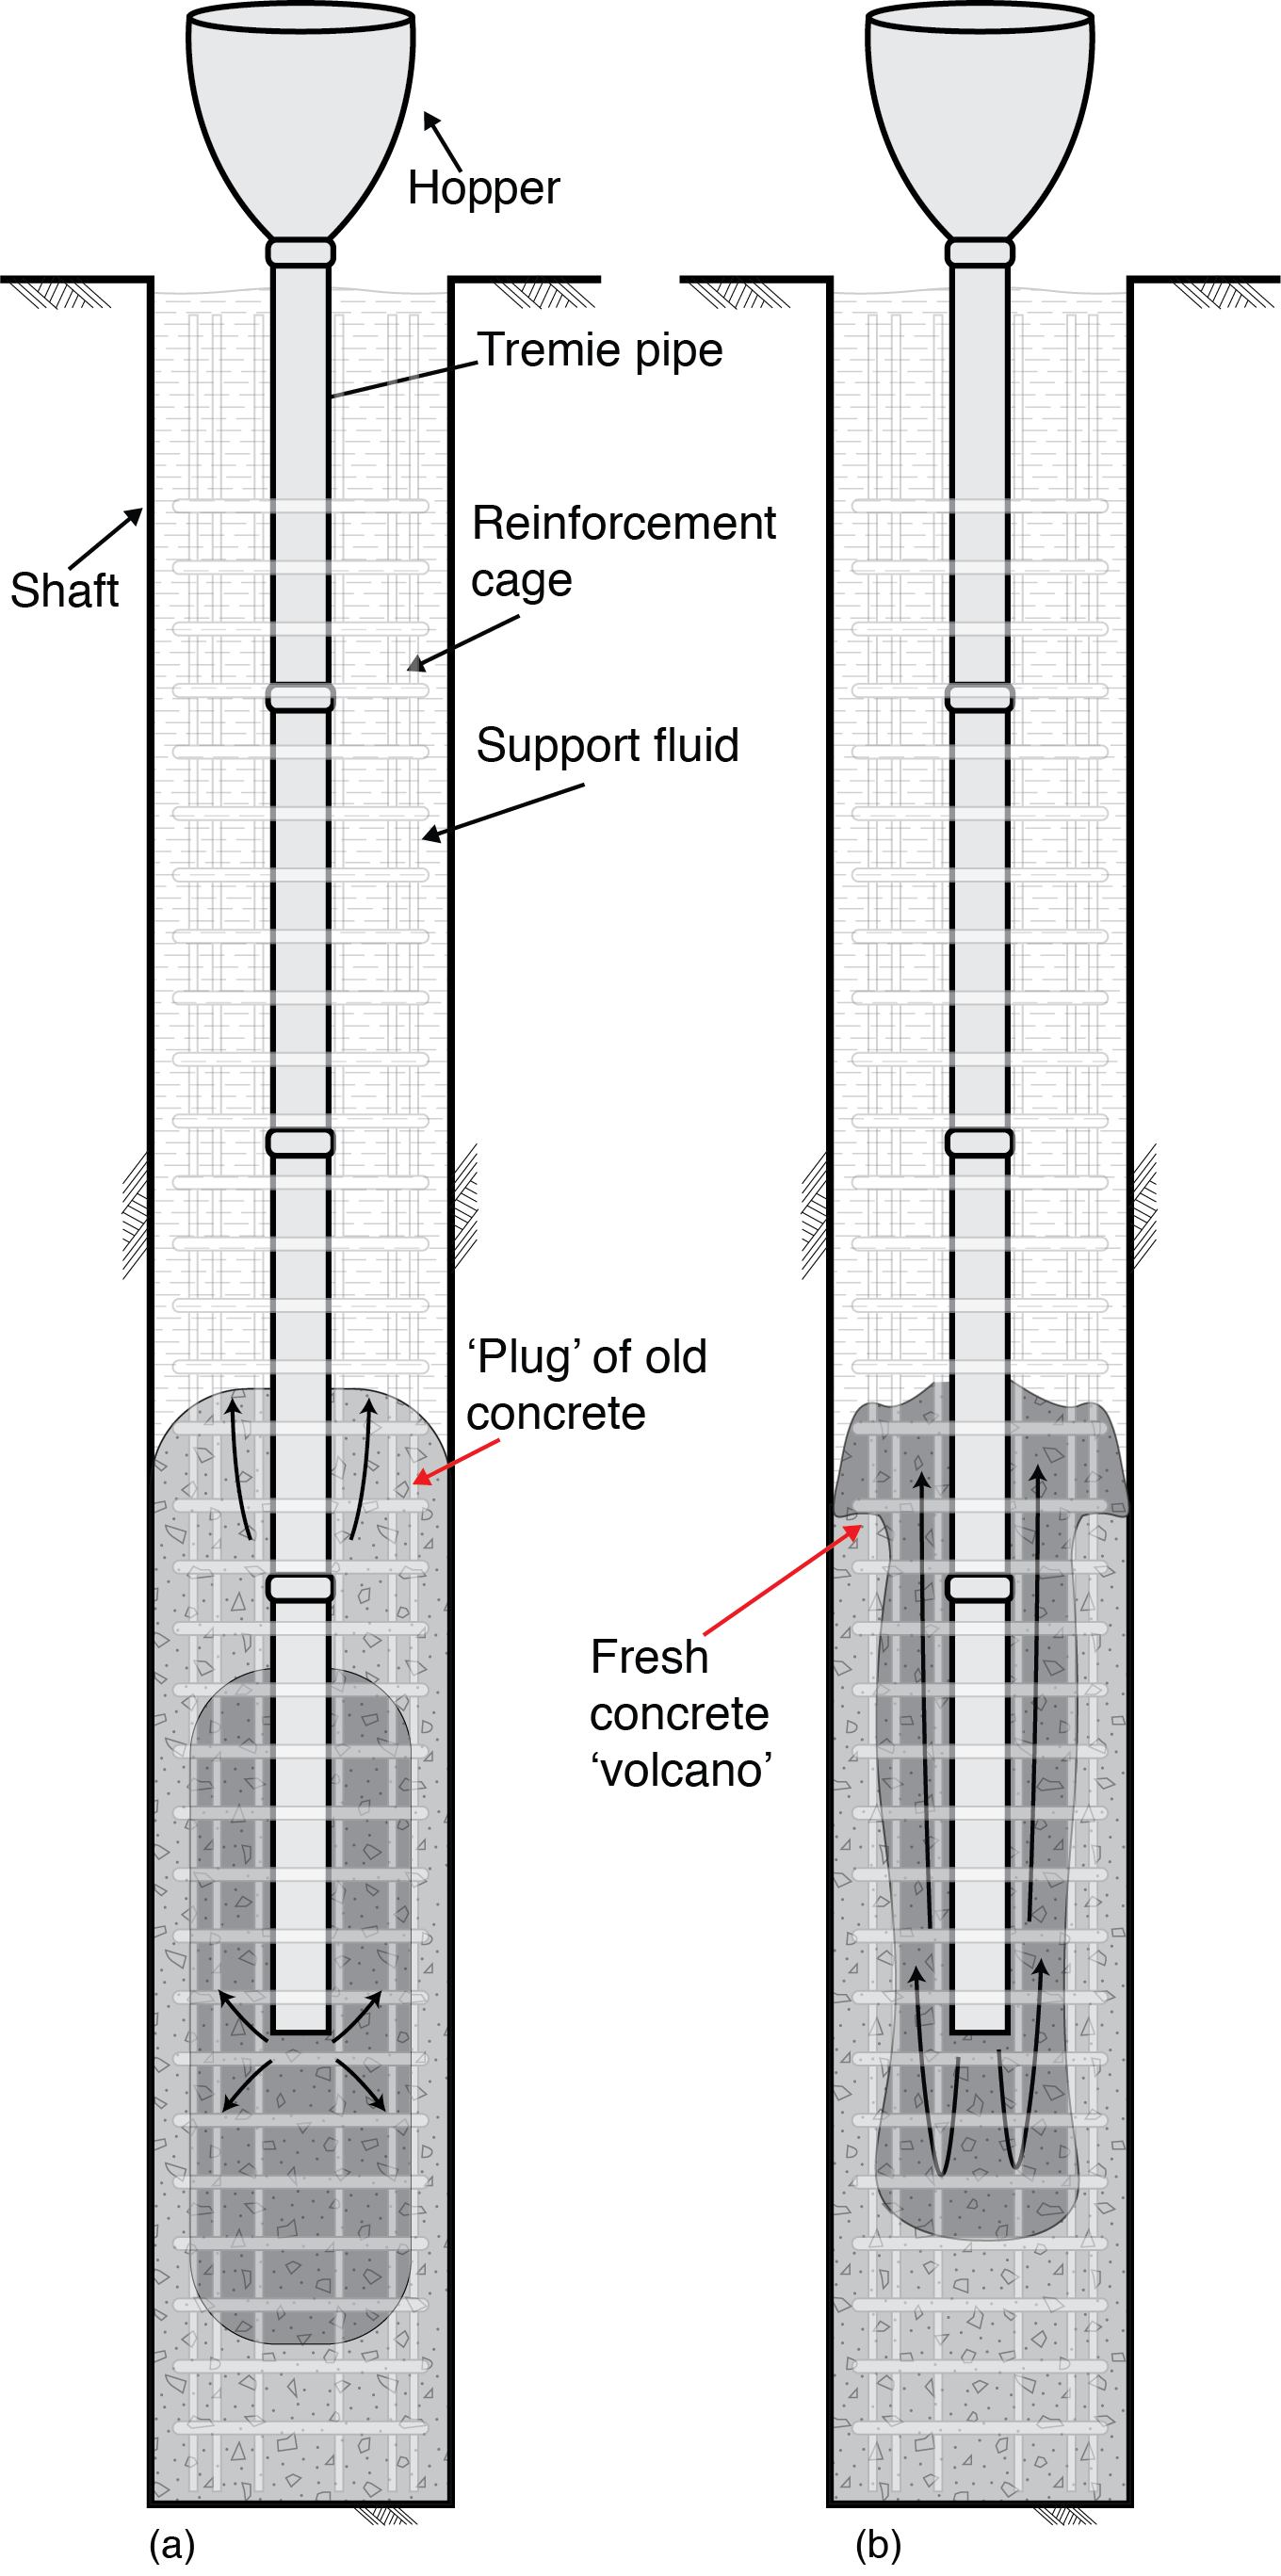
\includegraphics[width=0.7\textwidth]{flow_pattern_newstyle.png}
\caption{\label{fig:flowpattern}Schematic pile diagram showing a) theorised plug flow, where old concrete rises above fresh, and b) fresh concrete erupting at surface, referred to as volcano flow.}
\end{figure}

\begin{figure}[H]
\centering
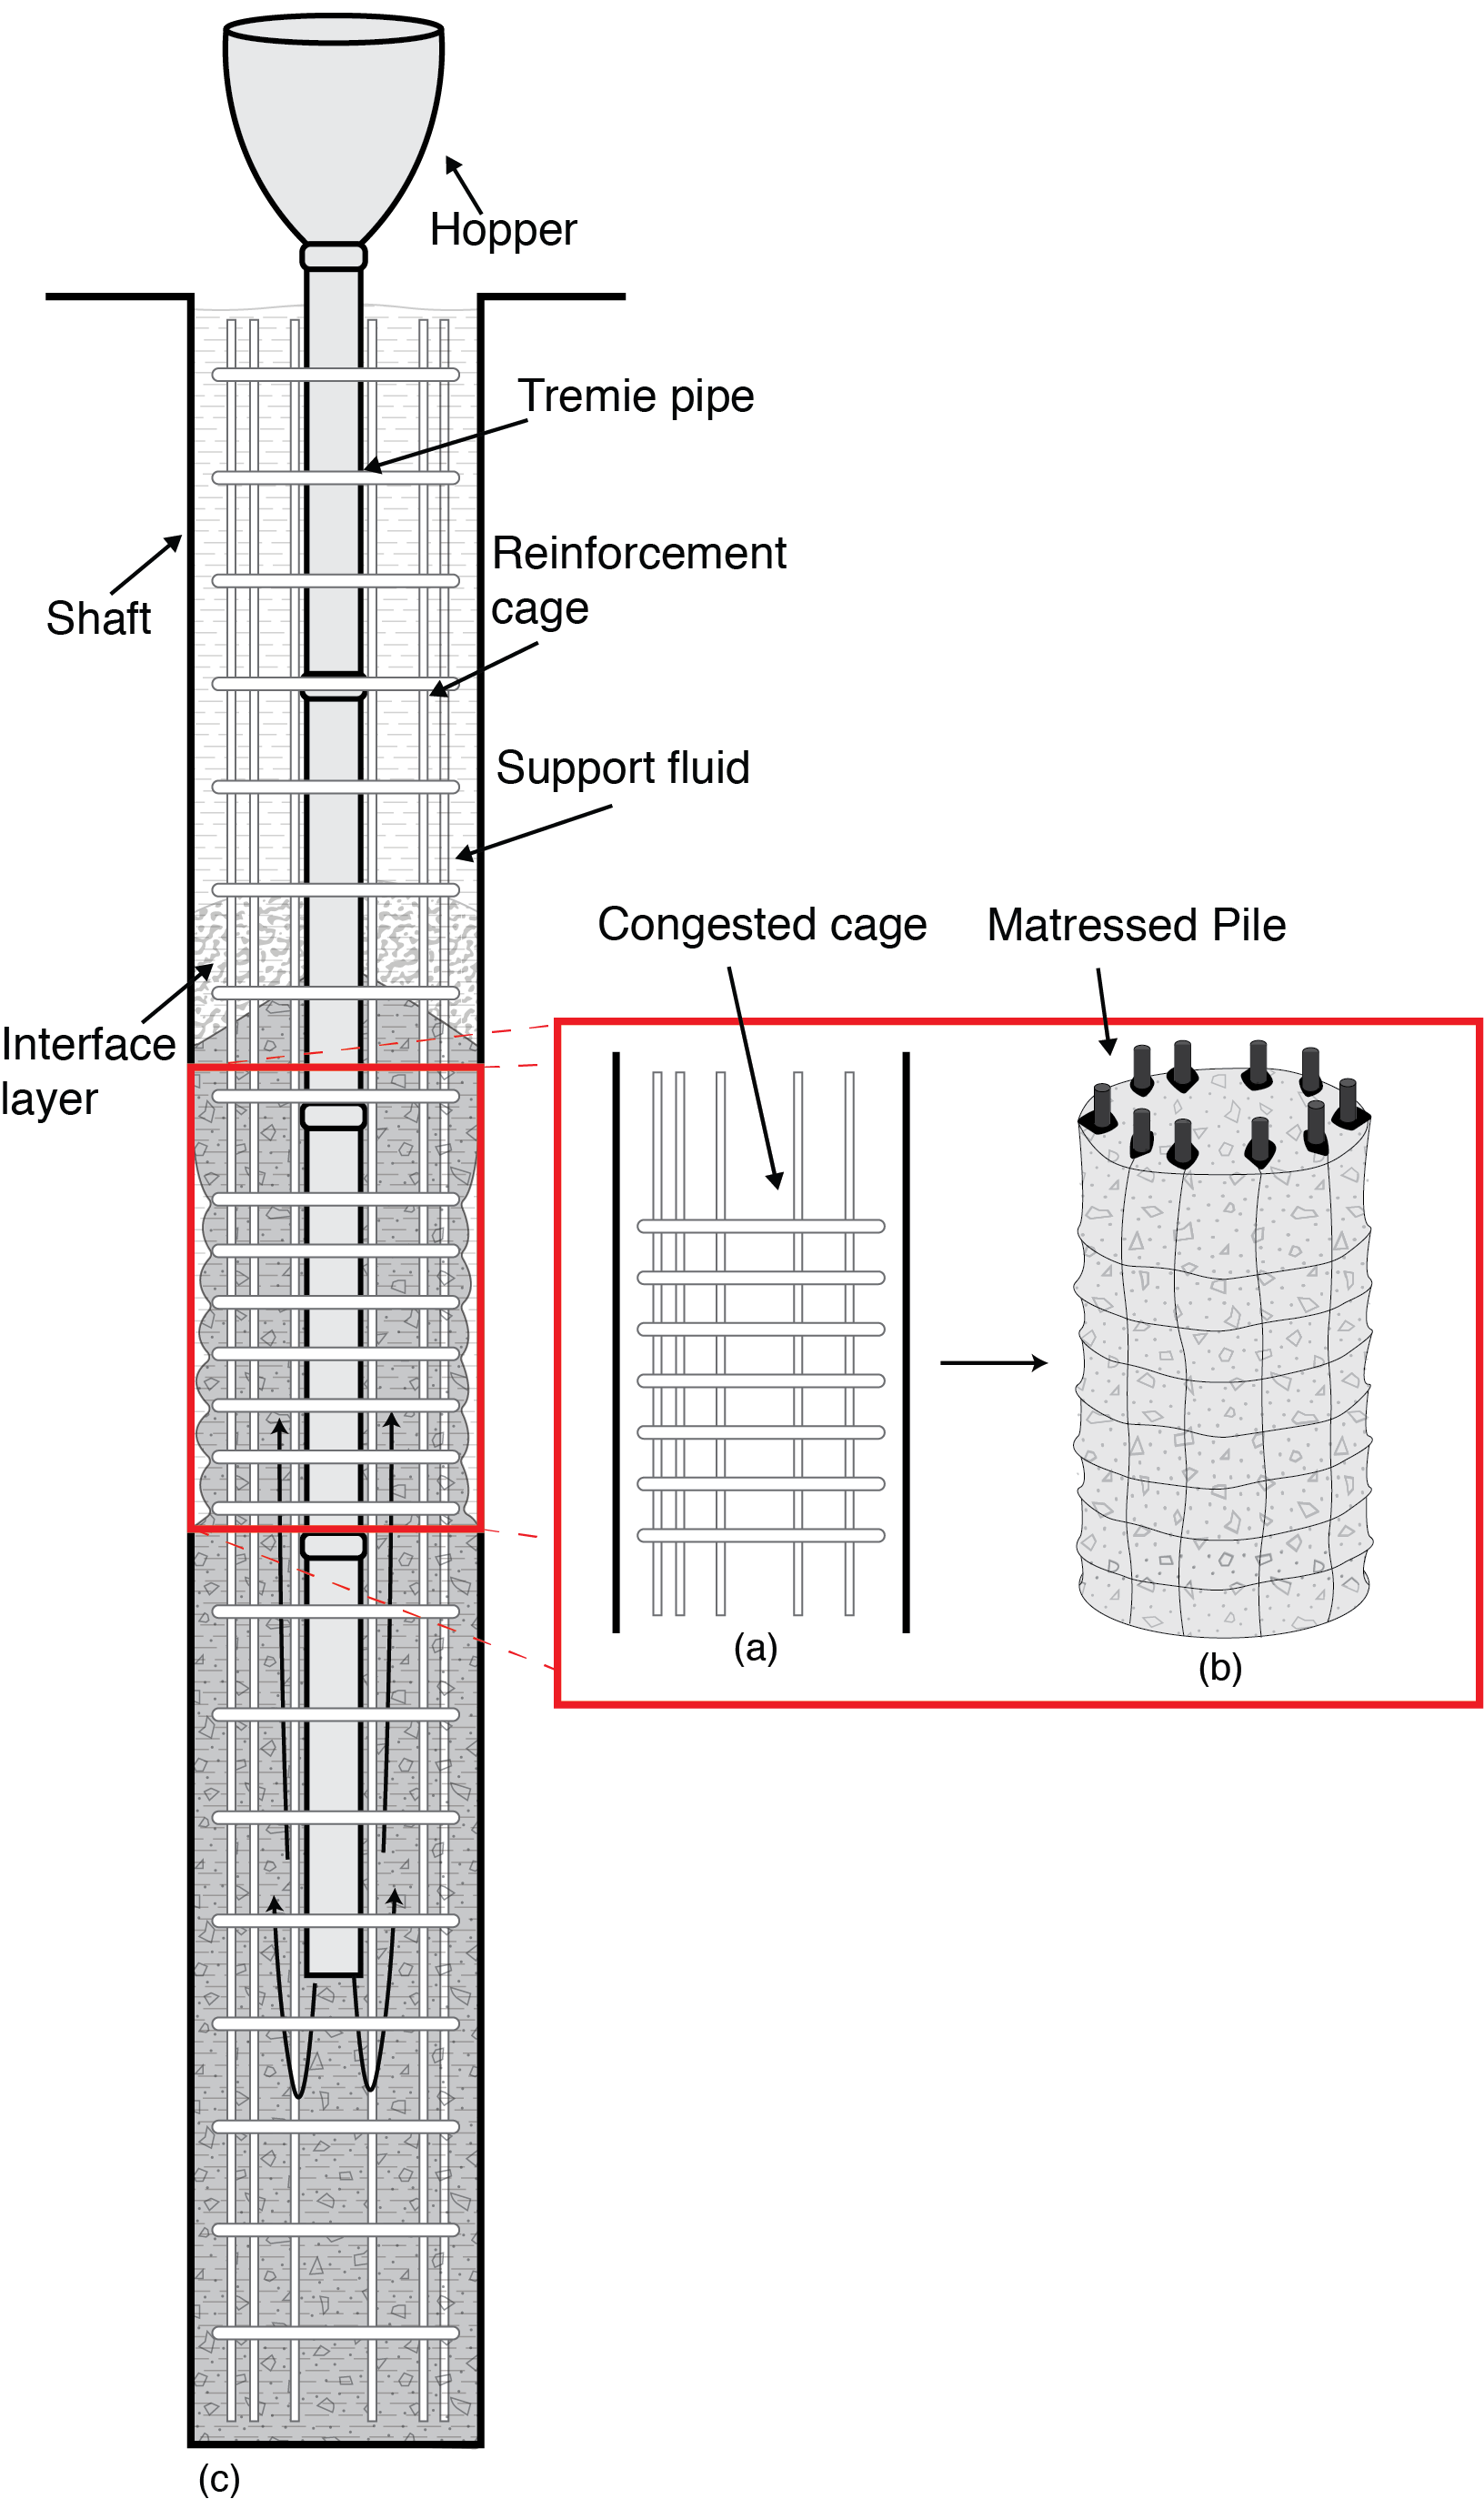
\includegraphics[width=0.8\textwidth]{matress.png}
\caption{\label{fig:matress}Diagram showing how a congested cage (a) could lead to a matressing effect on a a pile (b). c) Demonstrates that matressing likely to occur towards top of pile due to reduction in hydrostatic pressure.}
\end{figure}

\subsection{Bleed and Segregation}

Bleed and segregation issues within a cast in situ deep foundation can be extremely detrimental to the foundation. Mitigating the development of bleed within a pile should be a primary concern for the contractor, to prevent segregation occurring. Nonetheless, establishing when bleed has occurred or will occur is contentious. \citetex{EFFC} stipulate measures should be taken to avoid bleed and segregation, suggesting the material properties of the concrete have a direct baring on the likelihood of segregation. Simulations of varying properties may help provide guidance on acceptance criteria for concrete such that the effects of bled and segregation could be minimised.

%_****************************** SIMULATIONS ********************************************

\section{Concrete Simulations}
\noindent
Selecting a correct numerical method is tantamount to selecting a correct rheological representation. The early works of \citet{roussel07} lay the foundations for a more comprehensive review presented by \citet{sofcf} on the use of numerous possible methods for simulating concrete. This subsection aims to present the findings from both these reviews and of the surrounding literature in order to offer an informed decision on which method may be most suitable.\\
\newline
\noindent
The review presented by \citet{roussel07} details the potential models to select from; the Finite Element Method (FEM), Computational Fluid Dynamics (CFD), the Discrete Element Method (DEM) and a variation of the Material Point Method (MPM). Each potential method categorised by the form in which the material is represented.  FEM and CFD offer single fluid representation, whilst DEM offers a particulate representation. The version of MPM presented is able to represent concrete as a set of particles suspended in a fluid \citep{dufour05}.\\
\newline
\noindent
Computational Fluid Dynamics (CFD) is the part of fluid mechanics that refers to the use of numerical methods and algorithms to solve fluid flow problems; typically Eularian and single-phase in its approach. Using the most general description of a fluid flow, Navier Stokes Equations, mass conservation, conservation of momentum and conservation of energy are obtained \cite{tich15}. CFD is characterized by a coordinate system that is either stationary or moving in order to accommodate the continually changing domain. The mass travels between computational cells even if the grid moves, because grid movements are not related to the motion of the mass.\cite{GRAM14} consider the main issue with their chosen CFD model to be defining the optimum strategy for interference tracking.\\
\newline
\noindent
Ostensibly, CFD appears to be an appropriate choice; economic computational speed and ability to use pre-developed software capable of modelling thixotropic conditions with ease. However, most available CFD packages will simulate concrete as a homogeneous single-phase fluid. This means CFD cannot simulate solid particle heterogeneous phenomena (such as segregation and passing ability). \citep{sofcf} conclude CFD is appropriate for a general overview agreeing with \citet{gram2011} that CFD does not present the optimum representation of concrete..\\
\newline
\noindent
Conversely, Lagrangian descriptions can naturally handle material interfaces and may be utilised to handle large deformation problems, a common method used in other numerical methods.\\ 
\newline
\noindent
As stated in the problem definition of this report, there is a need to represent concrete as more than just a single-fluid; Using the Finite Element Method alone will incur the same pitfalls as its singular fluid counterpart CFD \citep{sofcf} with the addition of element distortion. A pile-scale simulation will require concrete simulated to undergo large deformation, particularly with reference to contact with reinforcement bars. Due to the nature of FEM, when the material represented becomes distorted, elongation of elements can occur. This extreme elongation yields inefficacy and inaccuracies \citep{moresi03}. \\
\newline
\noindent
Particle based methods offer an attempt to mitigate element based problems, simulating the material as a granular media, rather than a continuum body. Depending on mix design, concrete is potentially controlled by granular like behaviour; making it necessary to investigate the DEM. The calculations performed in the DEM alternate between the application of Newton’s second law with respect to the particles and a force-displacement law at the contact point between particles. The force-displacement law is used to update the contact forces arising from the relative motion at each contact, while the Newton’s second law is used to determine the motion of each particle arising from the contact and body forces acting upon it. The contacts between two neighbouring particles occur only at a point \cite{TAN215} According to \cite{roussel07} this offers a disadvantage, as the true nature of these contacts can never truly be known. Despite \citet{roussel16} advising that slump-flow results from DEM are comparative to CFD and FEM, \citet{roussel06} advises that due to both computational complexity and scaling issues, DEM may not be viable in pile-scale simulations.\\
\newline
\noindent
\citet{ALYHYA17} offers a promising review of a particle method in the form of SPH (smoothed particle hydrodynamics). With early results indicating there may be a potential for future work to produce compelling results. There are however similar pitfalls to DEM, when scaling and complexity become an issue. \\
\newline
\noindent
An attempt to bridge the gap between single fluid and granular representation is presented by \citet{roussel07} in the form of the early work conducted by \citet{moresi03}. Centralised on the Material Point Method devised by \citet{sulsky94}, concrete is represented as particles suspended in a fluid. Although not directly MPM, the Finite Element Method with Lagrangian Integration Points (FEMLIP) offered the closest representation of a Bingham fluid \citep{sofcf} and promising slump-flow results \citep{moresi03,dufour05}. Using MPM to simulate a granular media \citet{Krishna} presents MPM as able to handle high deformation problems, further bolstering MPM as a viable method for simulation of the tremie process.\\
\newline
\noindent
To summarise, although single fluid and granular representation of concrete are adequate at modelling concrete, they are not optimum. Progressing with a method capable of simulating a multi-phase material (MPM) has the potential to supplant these more established methods, providing a greater insight into the tremie process. In conjunction, the degree of deformation required to be simulated further justifies the choice of MPM over traditional methods such as FEM.
%***************************** MPM ***********************************************
\section{MPM}
The Material Point Method \citep{sulsky94,sulsky95} involves a continuum body discretised into a finite set of points ({\bfseries figure \ref{fig:discrete}}) with deformations governed by Newtons Laws of Motion. It combines the Lagrangian approach of tracking points with the Eularian approach of maintaining a background grid on which the momentum equation of the point is calculated. This is in contrast to other mesh-less methods, wherein the equations of motion are solved on the points themselves \citep{Krishna,Samila}.
\begin{figure}[H]
\centering
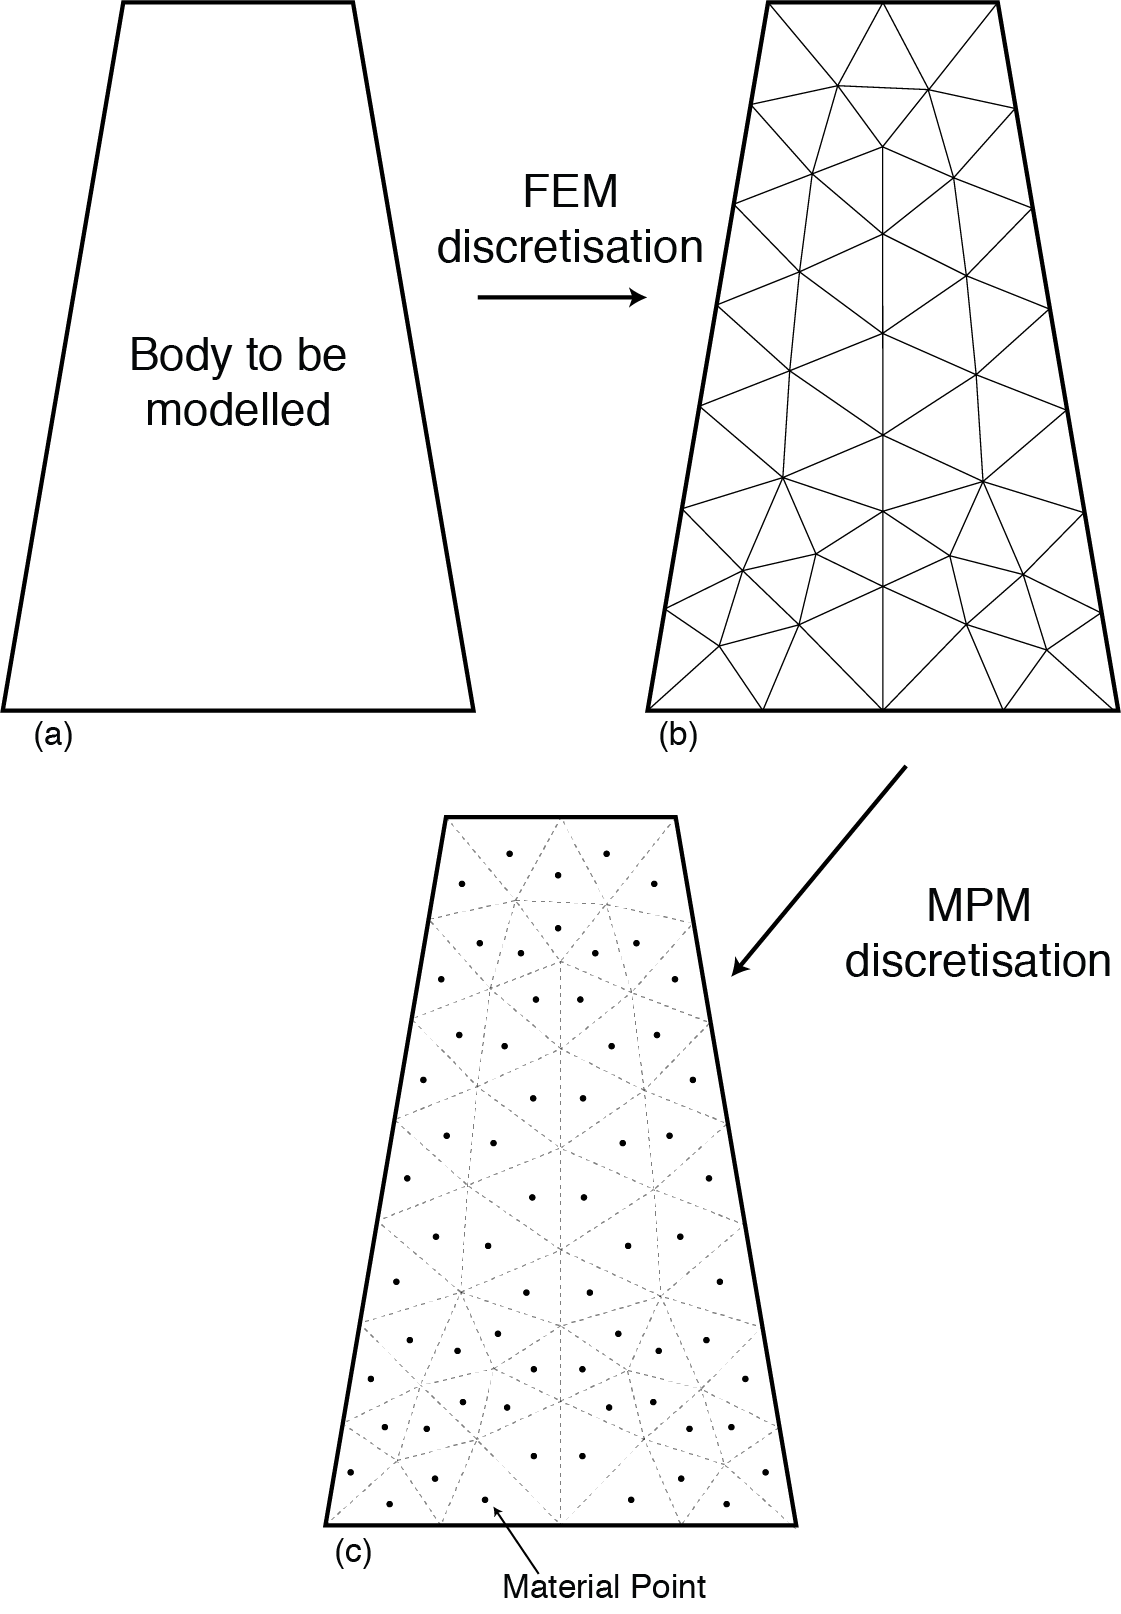
\includegraphics[width=0.65\textwidth]{discrete.png}
\caption{\label{fig:discrete}a) Body to be modelled b) the finite element method of discretising a body, c) the material point method of discretisation, extending from the FEM style.}
\end{figure}

\subsection{Governing Equations}
The governing equations are standard conservation equations for mass and momentum {\bfseries eq. \ref{eq:mass}} and  {\bfseries eq. \ref{eq:momentum}} respectivly. Derivations presented here are based on work conducted by \citet{sulsky95,Samila,Krishna,zhang16,Chen2002}
\begin{equation}
\frac{d\rho}{dt} + \rho\nabla\cdot \mathbf{v} = 0
\label{eq:mass}
\end{equation}
\begin{equation}
\rho a = \nabla\cdot\mathbf{\sigma} + \rho b
\label{eq:momentum}
\end{equation}
Let $\rho(\mathbf{x},t)$ represent the mass density of a point at location vector $\mathbf{x}$ and time $t$ such that $v(\mathbf{x},t)$ represents the velocity, $a(\mathbf{x},t)$ the acceleration, $\sigma(\mathbf{x},t)$ Cauchy's stress tensor and $b(\mathbf{x},t)$ the body force.\\
\newline
\noindent
Consider the finite number of points the continuum is divided into, to be represented by $n_p$. Let $\mathbf{x}_p^t$ represent the current position of point $p$ at time $t$ where $p=(1,2,...n_p)$. Each point at any given time will have an associated mass $m_p^t$, density $\rho_p^t$, velocity $\mathbf{v}_p^t$, and stress and strain $\mathbf{\sigma}_p^t$ \& $\epsilon_p^t$ respectively, providing a Lagrangian description of the body. Any parameters required by the chosen constitutive model, are also included. The values contained within the points are mapped onto the element nodes of the element they currently reside in.\\
\newline
\noindent
To obtain the discrete form of the equation, {\bfseries eq. \ref{eq:momentum}} is multiplied by weight function $w$ and integrated over boundary $\Omega$ to give
\begin{equation}
\int_\Omega \rho w \cdot ad\Omega = \int_\Omega w\nabla\cdot\sigma d\Omega + \int_\Omega \rho w b d\Omega \,.
\label{eq:weightfunction1}
\end{equation}
After integration by parts, the central term of {\bfseries eq. \ref{eq:weightfunction1}} becomes
\begin{equation}
\int_\Omega w\nabla\cdot\sigma d\Omega= \int_\Omega\nabla\cdot (w\sigma) d\Omega- \int_\Omega \nabla w\cdot\sigma d\Omega \,,
\label{eq:integrationbyparts2}
\end{equation}
where the central term of {\bfseries eq. \ref{eq:integrationbyparts2}} becomes
\begin{equation}
\int_\Omega\nabla\cdot (w\sigma) d\Omega= \int_{\partial\Omega} w \sigma \cdot n dS
\label{eq:divergence}
\end{equation}
because of the divergence theorem. $n$ represents the normal to the boundary.\\\\The right hand side of {\bfseries eq. \ref{eq:divergence}} represents the boundary term such that
\begin{equation}
\int_{\partial\Omega} w \sigma \cdot n dS = \int_{\partial\Omega_t} w\sigma\cdot n dS + \int_{\partial\Omega_u} w\sigma\cdot n dS \,,
\label{eq:boundary1}
\end{equation}
but owing to Nueman boundary conditions
\begin{equation}
\sigma(x,t)\cdot n = \tau(t) \text{ on } \partial\Omega_t
\label{eq:neumen}
\end{equation}
and test function $w$ being zero on Direchlet boundary $\partial\Omega_u$, {\bfseries eq. \ref{eq:boundary1}} becomes
\begin{equation}
\int_{\partial\Omega} w \sigma \cdot n dS = \int_{\partial\Omega_t} w\cdot\tau  dS
\label{eq:substitute}
\end{equation}
where $\tau$ represents surface traction.\\\\
Substituting {\bfseries eq. \ref{eq:substitute}} into {\bfseries eq. \ref{eq:integrationbyparts2}} gives
\begin{equation}
\int_\Omega w\nabla\cdot\sigma d\Omega= \int_{\partial\Omega_t} w\cdot\tau dS - \int_\Omega \nabla w\cdot\sigma d\Omega
\label{eq:substitute2}
\end{equation}
and substituting  {\bfseries eq. \ref{eq:substitute2}} into {\bfseries eq. \ref{eq:weightfunction1}} gives the final weak form of the equation of motion:

\begin{equation}
\int_\Omega \rho w \cdot ad\Omega =  \int_{\partial\Omega_t} w\cdot\tau dS - \int_\Omega \nabla w\cdot\rho\sigma^s d\Omega + \int_\Omega \rho w b d\Omega \,.
\label{eq:weakform}
\end{equation}
Where $\rho\sigma^s$ represents the the specific stress ($\sigma^s = \sigma / \rho$) necessary for the derivation of discrete equations, and $dS$ and $d\Omega$ represent surface and volume differential respectively. {\bfseries eq. \ref{eq:mass}} is automatically satisfied as material points have a fixed mass at all times.\\
\newline
\noindent
As the material is discretised into points, the mass density can be written as
\begin{equation}
\rho(\mathbf{x},t) = \sum_{p=1}^{n_p} m_p \delta(\mathbf{x-x}_p^t)
\label{eq:dirac}
\end{equation}
Where $\delta$ represent the Dirac delta function.\\
\newline
\noindent
Substituting {\bfseries eq. \ref{eq:dirac}} into {\bfseries eq. \ref{eq:weakform}} converts integrals to sums of quantities evaluated at material points, giving
\begin{equation}
\begin{aligned}
\sum_{p=1}^{n_p} m_p [w(\mathbf{x}_p^t,t)\cdot \mathbf{a}(\mathbf{x}_p^t,t)] = \sum_{p=1}^{n_p} m_p [-\sigma^s (\mathbf{x}_p^t,t)\nabla w \rvert_{\mathbf{x}_p^t}\\  + w(\mathbf{x}_p^t,t) \cdot \tau^s(\mathbf{x}_p^t,t)h^{-1} + w(\mathbf{x}_p^t,t) \cdot b(\mathbf{x}_p^t,t)]
\label{eq:sum1}
\end{aligned}
\end{equation}
where $h$ is the thickness of the boundary layer upon which the traction boundary conditions are enforced.\\
\newline
\noindent
Continuing discretisation, the coordinates of any material point located within an element of the background mesh can be represented as
\begin{equation}
\mathbf{x}_p^t = \sum_{i=1}^{n_n} \mathbf{x}_i^t N_i(\mathbf{x}_p^t)
\label{eq:shapefunction}
\end{equation}
where spacial nodes are represented as $\mathbf{x}_i^t$ such that node number $i = (1,2...n_n)$ with $n_n$ representing the number of nodes in the element. The element shape determined by background mesh governs the applied basis function $N_i$ similar to a finite element implementation. Velocity and acceleration also have a similar representation,
\begin{equation}
\mathbf{v}_p^t = \sum_{i=1}^{n_n} \mathbf{v}_i^t N_i(\mathbf{x}_p^t)
\label{eq:velocity}
\end{equation}
\begin{equation}
\mathbf{a}_p^t = \sum_{i=1}^{n_n} \mathbf{a}_i^t N_i(\mathbf{x}_p^t)
\label{eq:acceleration}
\end{equation}
as does the weight function
\begin{equation}
\mathbf{w}_p^t = \sum_{i=1}^{n_n} \mathbf{w}_i^t N_i(\mathbf{x}_p^t) \,.
\label{eq:weight}
\end{equation}
Substituting {\bfseries eq. \ref{eq:acceleration}} and {\bfseries eq. \ref{eq:weight}} into {\bfseries eq. \ref{eq:sum1}} and evaluating at time $t$ gives
\begin{equation}
\begin{aligned}
\sum_{i=1}^{n_n}w_i^t \cdot \sum_{j=1}^{n_n}m_{ij}^t \mathbf{a}_j^t = -\sum_{i=1}^{n_n} w_i^t \cdot \sum_{p=1}^{n_p} m_p \sigma_p^{s,t} \cdot \nabla N_i(\mathbf{x}) \rvert_{\mathbf{x} = \mathbf{x}_p^t} \\ + \sum_{i=1}^{n_n}w_i^t \cdot \sum_{p=1}^{n_p} m_p N_i(\mathbf{x}_p^t)\tau_p^{s,t} h^{-1} + \sum_{i=1}^{n_n}w_i^t \cdot \sum_{p=1}^{n_p}m_p\mathbf{b}_p^t N_i(\mathbf{x}_p^t) \,.
\label{eq:sum2}
\end{aligned}
\end{equation}
{\bfseries Eq. \ref{eq:sum1}} includes the addition of nodal mass matrix $m_{ij}^t$, 
\begin{equation}
m_{ij}^t = \sum_{p=1}^{n_p} m_p N_i(\mathbf{x}_p^t)N_j(\mathbf{x}_p^t)
\label{eq:massmatrix}
\end{equation}
and the specific stress at a point represented by
\begin{equation}
\label{eq:specstress}
\sigma_p^{s,t} = \sigma^s(\mathbf{x}_p^t,t)\,.
\end{equation}
{\bfseries Eq. \ref{eq:sum2}} can be further reduced to
\begin{equation}
\label{eq:reduced1}
\sum_{j=1}^{n_n} m_{ij}^t\mathbf{a}_j^t = \mathbf{f}_i^{int,t} + \mathbf{f}_i^{ext,t} \,.
\end{equation}
Where internal force vector is written as
\begin{equation}
\mathbf{f}_i^{int,t} = -\sum_{p=1}^{n_p} m_p \sigma_p^{s,t} \cdot \nabla N_i(\mathbf{x}) \rvert_{\mathbf{x} = \mathbf{x}_p^t}
\label{eq:internal}
\end{equation}
and external written as
\begin{equation}
\mathbf{f}_i^{ext,t} = \sum_{p=1}^{n_p} m_p N_i(\mathbf{x}_p^t)\tau_p^{s,t} h^{-1} + \sum_{p=1}^{n_p}m_p\mathbf{b}_p^t N_i(\mathbf{x}_p^t) \,.
\label{eq:internal}
\end{equation}
\newline
\noindent
Boundary conditions are evoked when a particle falls within a boundary cell, if multiple cells are located within a boundary cell, they are treated as boundary points. \citet{Krishna} suggests maintaining a smaller mesh at boundaries may be beneficial. A modified frictional algorithm based on the work of \citet{Krishna} and \citet{Samila} is presented later in this report. Integrations and solution schemes are also detailed later in this report.
%******************************************* EXPLICIT *************************

\subsection{Explicit Material Point Method}

The equation of momentum {\bfseries eq \ref{eq:momentum}} is a second-order differential equation with respect to time and can be solved by using either an explicit integration scheme or an implicit integration scheme. The explicit integration scheme finds the state variable 
\begin{equation}
y(t+\delta t) \,,
\label{eq:explicit}
\end{equation}
at the next time-step based on the state variable $y(t)$ at the current time-step. The implicit scheme finds the state variable {\bfseries eq \ref{eq:explicit}} by solving the equation:
\begin{equation}
G(y(t),y(t\delta t))  = 0\,.
\label{eq:implicit}
\end{equation}
{\bfseries Eq \ref{eq:implicit}} uses both the current and later state variables \citep{zhang16}. For a scenario involving a slowly applied and propagated stress \citep{kafaji13} infers the use of an implicit time integration scheme will reduce computational time. The high stability of an implicit time integration scheme is presented by \cite{love06}, but owing to rapid application of forces required to simulate the tremie process, and explicit time integration scheme must be adopted.\\
\newline
\noindent
All material properties within MPM are carried by points and mapped onto nodes. Therefore, no permanent information is stored at nodes. Point values are projected onto the nodes using the shape functions derived from the particle position within the grid \citep{Krishna}. After solving the grid nodal momentum equation with an explicit time integration scheme, the grid nodal acceleration and velocity values are mapped back to the points to update their velocities and positions \citep{zhang16}. The stress of a point can be further updated using a constitutive model. The update to the stresses can be implemented either by updating stresses first (USF scheme) or updating stresses last (USL scheme). \citet{nairn03} observed that USL has serious numerical difficulties which are due to considering a node which interacts with only a single particle. Whereas, \citet{bardenhagen02} proposed USL performed better than USF. \cite{kafaji13} Supports the use of USL over USF on the basis that it dissipates energy as opposed to USF which gains energy.\\
\newline
\noindent
\citet{nairn03} offers a potential solution to the energy dissipation or creation dilemma. Proposing a modified updated stress last scheme (MUSL). In USL, grid nodal velocity from the updated momentum is used to update the stress state. In the MUSL scheme, the grid nodal velocity obtained by mapping the updated point momentum back to the grid nodes is used to update the stress state. The USF and MUSL schemes are similar in their implementation, but MUSL is observed to maintain conservation. USL is chosen by \citet{Krishna} as a preferred method for the simulation of granular problems, therefore this present study will also use the USL method.
\subsection{Algorithm}
{\bfseries Figure \ref{fig:nodal}} is a visualisation of the algorithm used in MPM... solution scheme detailed here.

\begin{figure}[H]
\centering
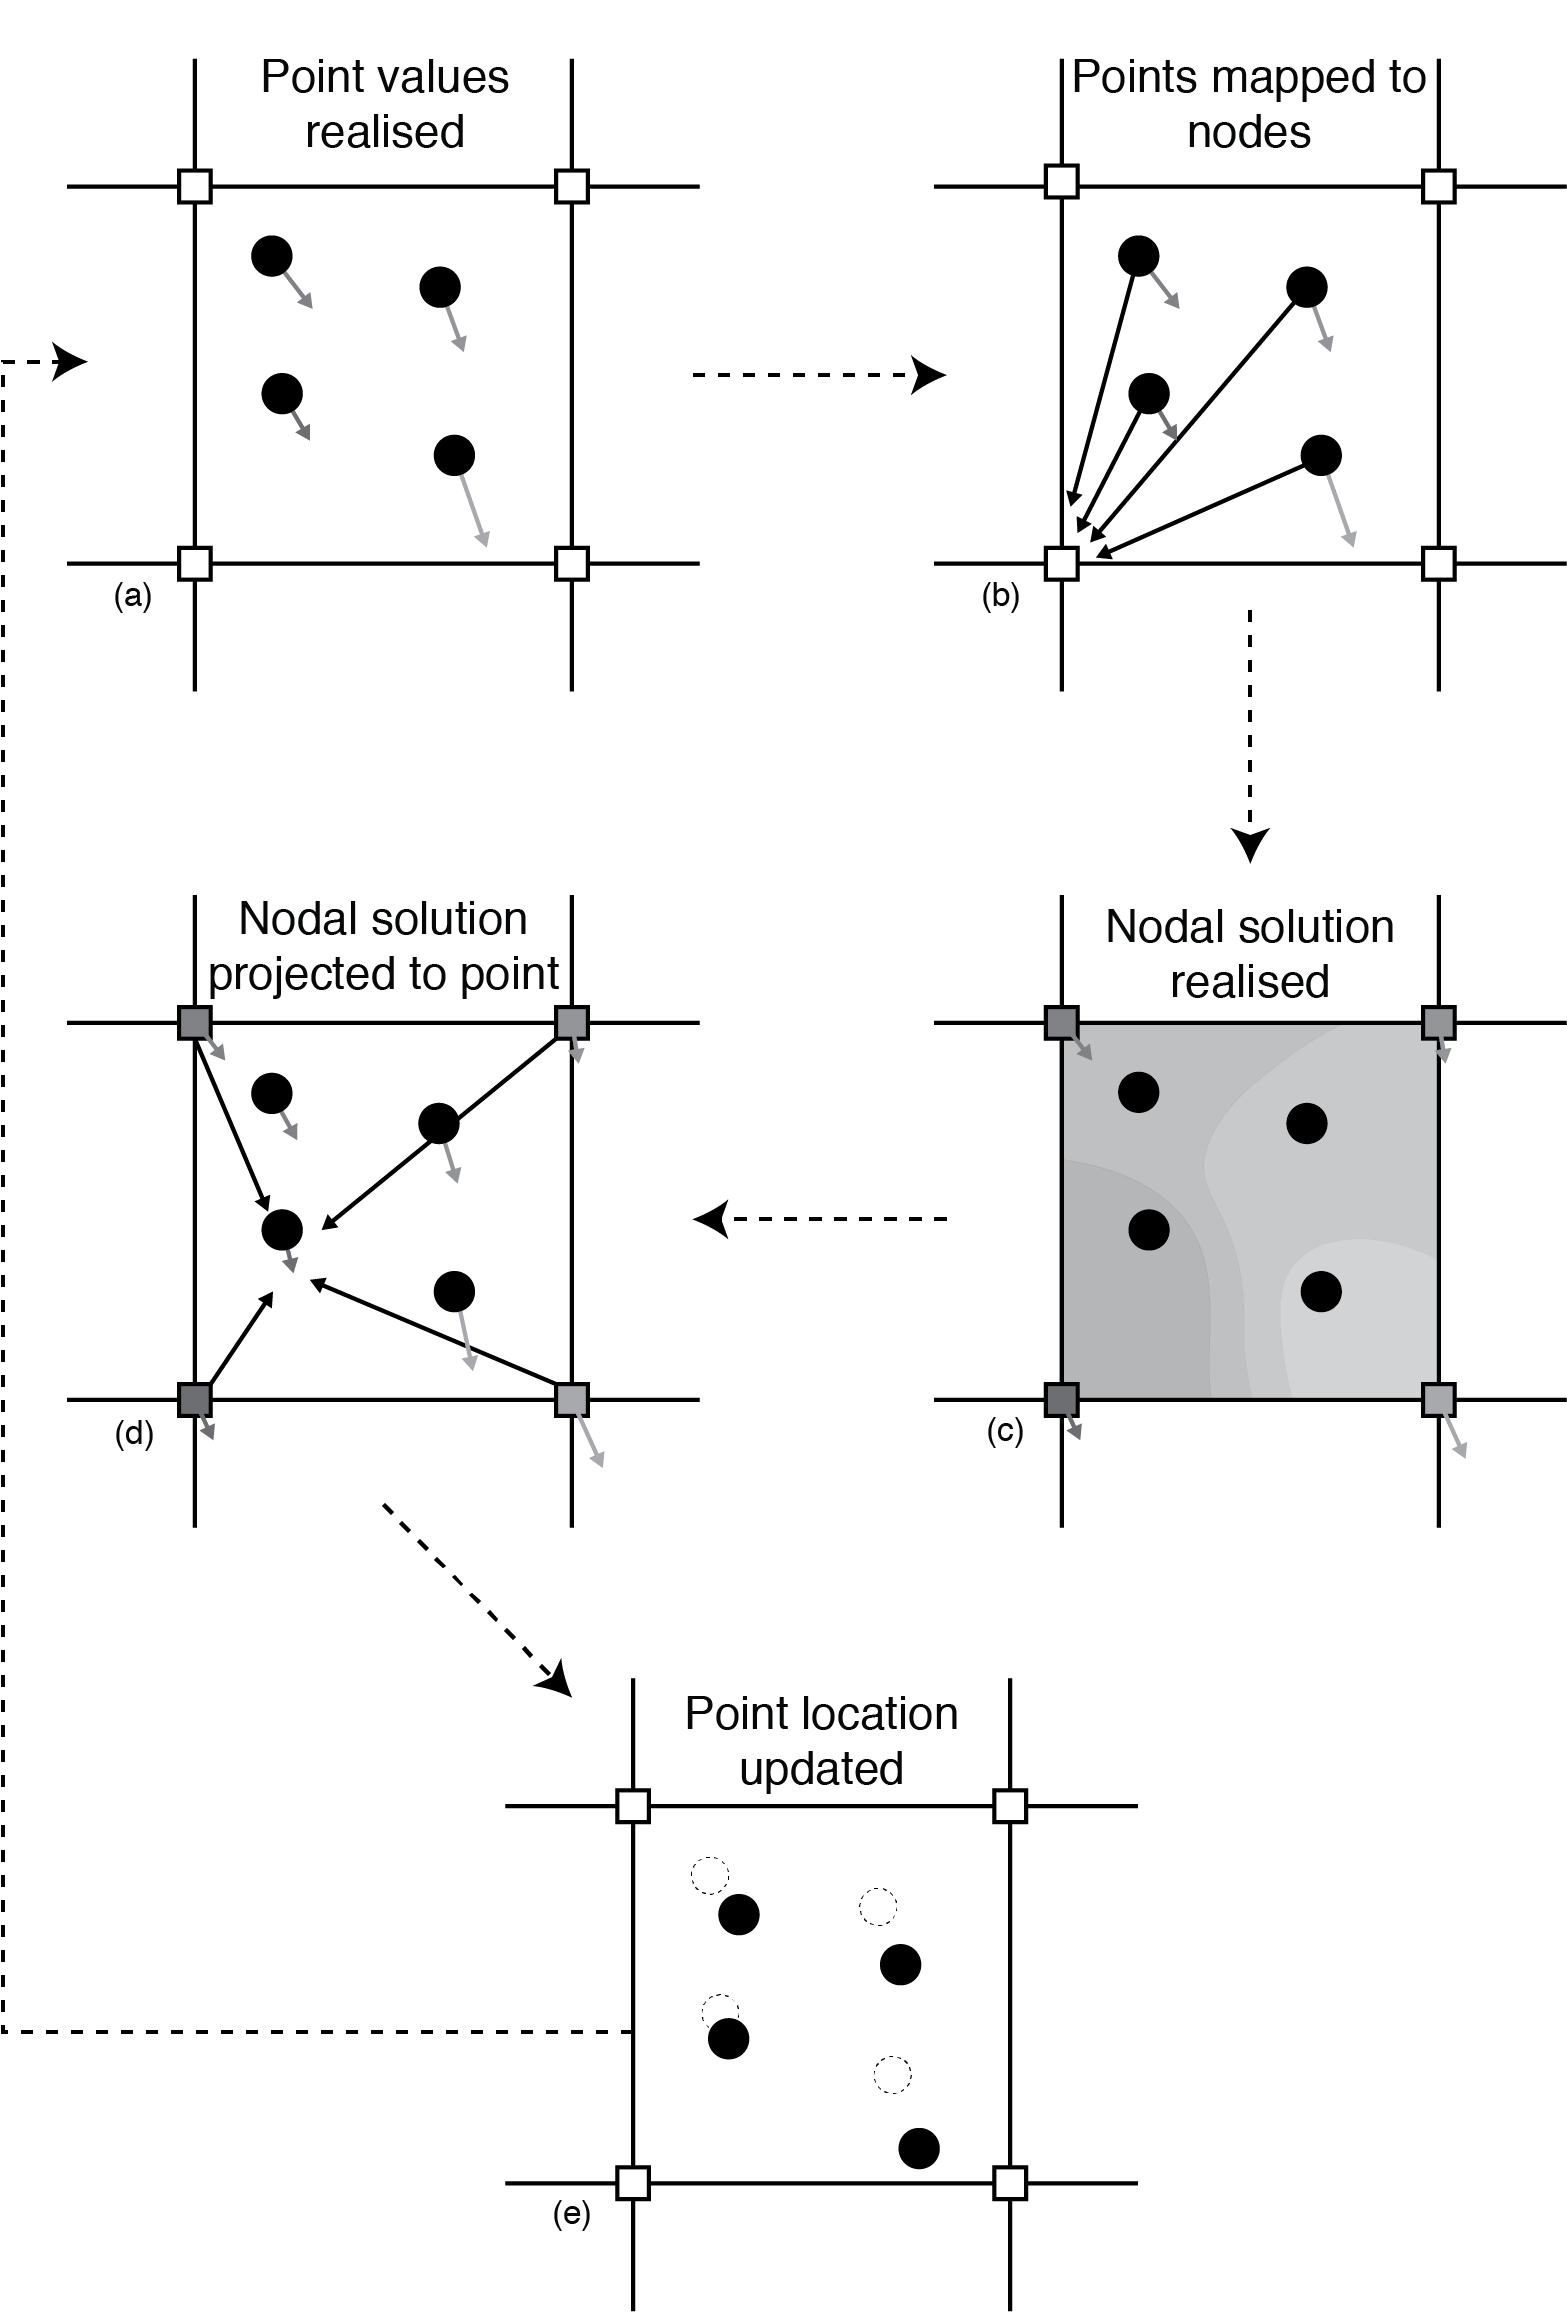
\includegraphics[width=0.85\textwidth]{nodal.png}
\caption{\label{fig:nodal}Schematic diagram of the material point algorithm, arrows represent material point properties (velocity, mass etc.) a) Point values are initialised b) Point values are mapped to nodes c) The equations of momentum are solved on the nodes d) Updated Nodal values are projected back to points e) Point locations and states are updated.}
\end{figure}

\subsection{GIMP}
GIMP equation and figure. Cell crossing also included.





